%************************************************
\chapter{Session tracking}\label{p02:session_tracking}
%************************************************

In order to understand the learning process, we need to keep track of the working sessions. The term refers to either reading or exercising sessions. A reading session is considered as an uninterrupted reading activity of a particular article. A similar concept applies for exercises, except that they can encompass multiple articles. Given the fact that students can switch between windows or even walk away from the screen, a method to compute the effective working time is devised. 

\section{Algorithm}
The algorithm to compute the reading session works under the assumption that all user actions fall under one out of three types: opening, interaction or closing events.

By following the Markov model on figure \ref{fig:markov_diagram}, we observe that depending on the type of event, a working session can be either created, updated (kept alive) or closed. With this simple approach, the algorithm can be fine tuned by adding or removing events (\Eg including the scrolling as a interaction event).

\begin{figure}[bth]
	{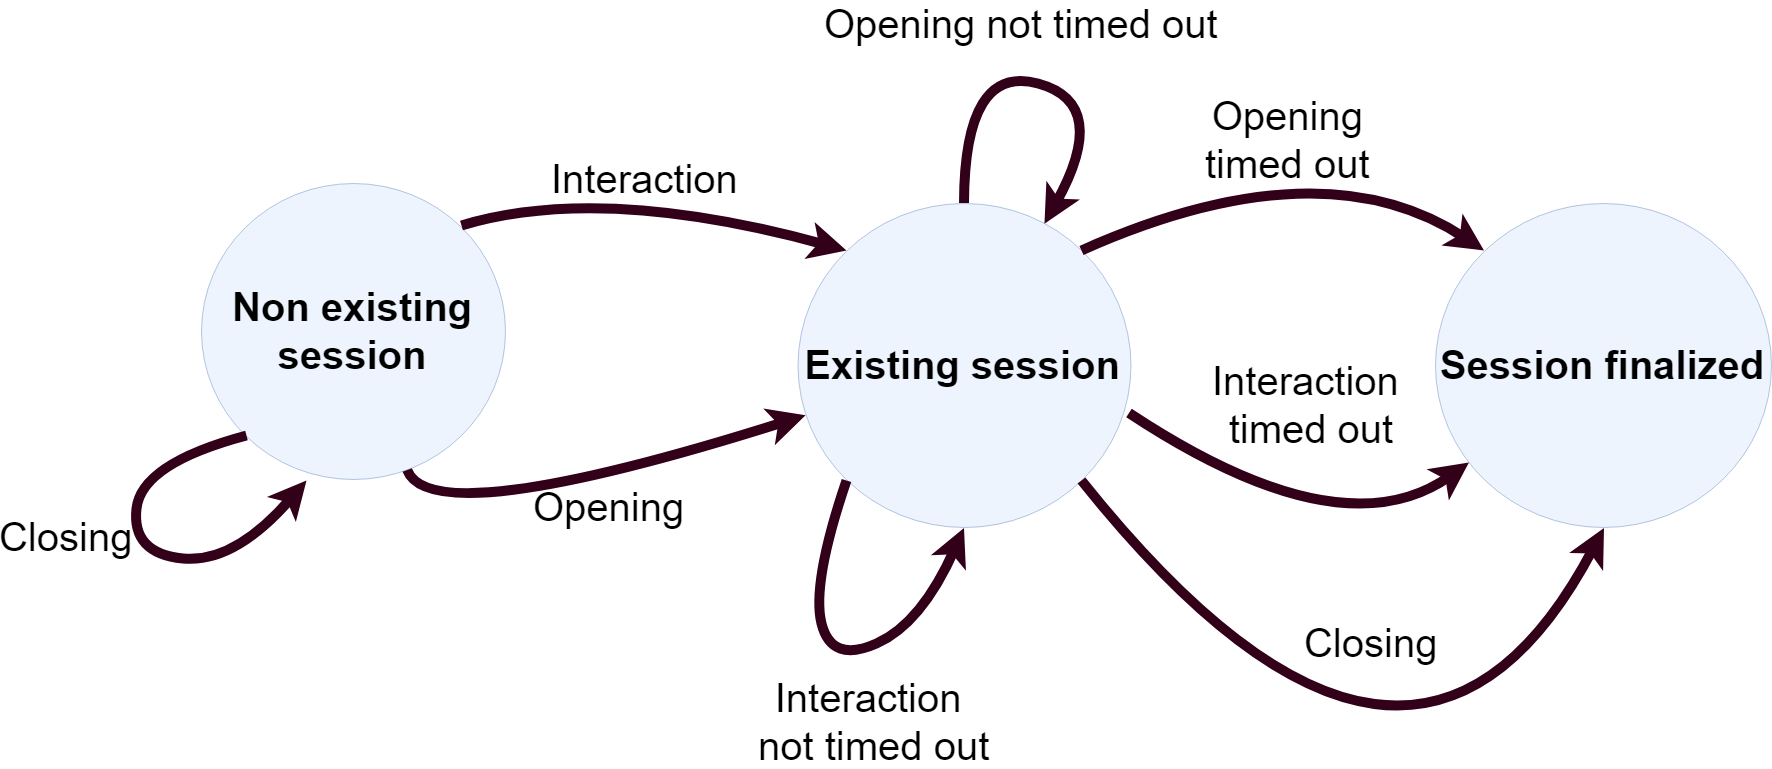
\includegraphics[width=1\linewidth]{gfx/Finite_state_machine_diagramv2}} \quad
	\caption[Finite state diagram - Working session transitions due to user actions]{Finite state diagram - Working session transitions due to user actions}\label{fig:markov_diagram}
\end{figure}

Additionally, there is a \textbf{session\_timeout} parameter which is used to handle scenarios where a session was not properly closed (\Eg when the browser was closed or the computer was turned off). The parameter is used in 2 different situations:

\begin{itemize}
	\item When the user is inactive for a long period, the session is closed and a bonus of "+ session\_timeout" minutes are added to the last action date and time. Under the assumption that the user did not stop working immediately after the last action.
	
	\item When the user is taking unusually too long between actions the activity is considered as suspicious and the session is closed. A new session is created with the next user action.
\end{itemize}


\section{Reading session}
With the help of Javascript code, user actions like opening an article, translating a word, or even switching the browser tab can be detected and tracked, however events like when the user abruptly closes the browser or turns of the computer, or even when the user walks away from the screen cannot be detected using Javascript. For these scenarios, a timeout parameter is used that finalizes the session after \textbf{N} number of minutes. If the timeout value is too small an advanced student that does not translate any word but reads a long text might be incorrectly measured, while if the value is too big, we would incorrectly consider longer reading sessions.

Some important assumptions for the implementation of the reading session are:
\begin{itemize}
\item Reading session are considered per article. Therefore, when the user closes and opens a new article we consider it as a new session. In this way we solve an issue where the same user could have open in different tabs different articles and switches between them.

\item For scenarios when the user leaves the session open for a time period longer than the session\_timeout, we give it a time benefit of “session\_timeout” minutes, because we cannot know exactly how long after the last action, the user kept reading. 

\item When the user opens a new article without closing the previous one(s) we close the other reading session(s) because the user is supposed to read one article at the time.

\item A user can read the same article multiple times, and each time is considered a new session (unless the time between both of them is less than the session timeout, in which case the two sessions are merged).
\end{itemize}

\section{Exercise session}
In the case of exercise sessions, the implementation is simpler, because the only possible interaction is answering either correctly or wrongly the exercise. 

Therefore, opening an exercise does not count for the active session, only answering. As long as the time between two exercises is smaller than the session\_timeout the exercises will be placed under the same exercise session.

For exercise sessions we can be more precise on the tracking because an exercise usually comes surrounded by a single sentence, therefore the timeout can be set to a smaller value. 

The final difference with the reading session is that no "benefit time" is granted to the user, the only actions that keep the session alive are answering the exercise.


%TODO explain events tracked and events that were added

%TODO explain script for historical data


%TODO Later, the implementation of the algorithm in the system, for this, it was needed to implement additional user actions detection (lost focus, and scrolling)